\documentclass[11pt,en]{elegantpaper}

\title{Privacy preserving health code app based on Tracking Code}
\author{Wangzhihui Mei 2019124044\ Hongyi Huang 2019124044 \ Zijia He 201912xxxx \ Chang Xu 201912xxxx\\ Zhanping Zhou 201912xxxx}
\institute{CCNU-UOW JI}

\version{}
\date{}


\begin{document}

\maketitle

\begin{abstract}
	At the critical moment of resisting COVID-19, in order to better block the transmission path of the virus and to better study the vaccine, it is very urgent to develop a reasonable virus tracing system\cite{guan2020clinical}. In view of the widespread use of "health codes", this paper proposes a more reasonable virus tracing system based on 3-phase code interaction technology. It is mainly constructed from short-distance bluetooth beacon data transmission and some encryption methods.
\end{abstract}

\section{Introduction}
At present, new coronavirus is rampant around the world, and the whole world is facing a huge storm. The cloud server should not be able to read person’s information Today, when medical technology is quite developed, the new coronavirus discovered for the first time in large-scale infections are still somewhat helpless.

At present, China has found a suitable and reasonable way to resist COVID-19, which is an excellent generic for other countries to refer to.

In order to effectively control the epidemic, China has not only continuously developed vaccines from the technical aspect, but also adopted a powerful political means: isolation. Quarantine greatly reduces the spread of the epidemic but the national economy cannot be paralyzed, and people need to resume work to maintain a normal order of life. In order to prevent the virus from spreading again, and in order to better trace the source of the virus infection, accelerate the research of the vaccine, it is very necessary to develop a reasonable traceability system.

The "health code", as a pass for returning personnel, records the individual's health and takes the form of "green code", "red code", and "yellow code" to dynamically detect data. The appearance of the "health code" relieves personnel from carrying out a series of complicated auditing methods and is a powerful anti-epidemic measure.

However, the "health code" still has the following problems:

\begin{itemize}
	\item First, whether users will be willing to record their personal information, that is, security issues: whether users are willing to expose their personal information to the company to which the "health code" belongs;
	\item Secondly, will users be willing to fill in the real information, that is, the problem of data authenticity: do not hide the report;
	\item Finally, how to continue to use its statistical data without exposing privacy, that is, statistical data openness
\end{itemize}

We use Wechat health code miniprogram as the tracking program.

Generally, We want to verify the fact whether the user has ever in close contact with infector. But we don't want the information of non-suspicious person to be leaked. 

\section{Virus tracing system protocol}
In this chapter, we mainly introduce the protocol framework of the virus tracing system.

\subsection{Demand analysis}
The application scenario firstly is going to be verified this section. Generally speaking, the Wechat platform is the container of the application. User data including ID number, location history and social connection can be fetched by related department such as department of health.

The typical scenarios are:
\begin{itemize}
	\item The personal information of users should be registered through Wechat platform, including: name, ID number, address, phone number and so on.
	\item when entering or leaving some specific areas current status(ID number, location, time, etc.) should be updated achieving by forcing the user to scan QR code.
	\item User information is uploaded and stored in the cloud server. If sometime later an infection source is pinpointed, the related information (the person within the limited range and time window) can be traced, so that the status of the related person’s health code should be turned to yellow or red instead of normal green.
\end{itemize}

In this situation, based on privacy protection, we treat server as untrusted terminal.\cite{berke2020assessing} Meanwhile, the epidemic prevention concern should be treated carefully. We want to guarantee:
\begin{itemize}
	\item The information exchanged itself is anonymous;
	\item Even if the privacy protection requirements are met, the information can still be decrypted when needed and the contact can be located.
	
\end{itemize}

\subsection{Proposed Protocols}

\subsubsection{Mathematic Detail}
% \textbf{HMAC}

% HMAC definition is taken from RFC 2104:
% $$HMAC(K,m)=H((K'\oplus opad)||H(K'\oplus ipad) || m)$$

% where $H$ is a cryptographic hash function, $m$ is the message to be authenticated, $K$ is the secret key, $K'$ is a block-sized key derived from the secret key.


\textbf{HKDF}

HKDF \cite{briefxip3322b}designates the HKDF function as defined by IETF RFC 5869, using the SHA-256 hash function: 
$$Output\leftarrow HKDF(key,Salt, Info, OutputLength)$$

\textbf{AES}

AES \cite{gueron2020flexible}designates the encryption of a single AES-128 block
$$Output\leftarrow AES_{128}(Key,data)$$

\textbf{CRNG}

The CRNG \cite{datcu2020chaos}function designates a cryptographic random number generator: 
$$Output\leftarrow CRNG(OutputLength)$$

\textbf{ENIntervalNumber}

ENIntervalNumber (ENIN) function provides a number for each 10 minute time window that’s shared between all devices participating in the protocol. These time windows are derived from timestamps in Unix Epoch Time. ENIN is encoded as a 32-bit unsigned little-endian value.

$$ENIN(timestamp)\leftarrow timestamp/(60\times 10)$$

\textbf{TEKRollingPeriod}

TEKRollingPeriod (TEKRP) is the duration for which a Temporary Exposure Key is valid (in multiples of 10 minutes). In our protocol, TEKRP is defined as 144, achieving a key validity of 24 hours. 

\textbf{Temporary Exposure Key}

When setting up the device for exposure detection, the first Temporary Exposure Key (tek) is generated on the device and associated with an ENIN , corresponding to the time from which the
key is valid. That value is aligned with the TEKRP and is derived as follows: 

$$i\leftarrow \lfloor ENIN(time_{keygen})/TEKRP\rfloor \times TEKRP$$

The devices generate the 16-byte Temporary Exposure Key as follows: 
$$tek_i\leftarrow CRNG(16)$$

The key is securely stored along with $i$. At the end of every TEKRollingPeriod, a new key is generated. 

\textbf{Rolling Proximity Identifier Key}

Rolling Proximity Identifier Key (RPIK) is derived from the Temporary Exposure Key and is used in
order to derive the Rolling Proximity Identifiers\cite{hirmer2020techniques}. 
$$RPIK_i\leftarrow HKDF(tek_i,NULL,UTF8(Info), 16)$$

\textbf{Rolling Proximity Identifier}

Rolling Proximity Identifiers are privacy-preserving identifiers that are broadcast in Bluetooth payloads.

Each time the Bluetooth Low Energy MAC randomized address changes, we derive a new Rolling
Proximity Identifier using the Rolling Proximity Identifier Key: 
$$RPI_{i,j}\leftarrow AES_{128}(RPIK_i,PaddedData_j)$$

The use of 16-byte identifiers yields a low probability of collisions, and limits the risk of false-positive matches, while keeping device storage requirements low. 

\textbf{Associated Encrypted Metadata Key}
The Associated Encrypted Metadata Keys (AEMK) are derived from the Temporary Exposure Keys in order to encrypt additional metadata.
$$AEMK_i\leftarrow HKDF(tek_i,NULL,UTF8(Info), 16)$$

\textbf{Associated Encrypted Metadata}
The Associated Encrypted Metadata (AEM) is data encrypted along with the Rolling Proximity Identifier, and can only be decrypted later if the user broadcasting it tested positive and reveals their Temporary Exposure Key\cite{keselman2020homomorphic}. 
$$AEM_{i,j}\leftarrow AES_{128}-CTR(AEMK_i,RPI_{i,j},Metadata)$$


\subsubsection{General Procedure}
There are three tracking code in the protocol\label{fig1}, we call them 3-phase code, which is the basic of the protocol. 

The first code is the Metadata Tracking Code or Temporary Exposure Key($tek$). It is generated from the Wechat client when the health code app is first opened. It is a Metadata and unique code that will never change. Meanwhile, it will never be shared to other clients or server and will just be stored securely in mobile phone. The code was generated from a Cryptography random number generator (CRNG):
$$tek = CRNG(32)$$

The $tek$ has nothing to do with the known identification code of users' mobile phone, such as serial number, MAC address, and will not be uploaded, so there is almost no privacy risk.

The second code is the Periodic Tracking Code or Associated Encrypted Metadata Key($aemk$). It is derived from the $tek$ using the HKDF function and is 32 bytes in length. Updated every 24 hours,

$aemk$ will not be uploaded when user is healthy. Only when the diagnosis is confirmed, the $aemk$ will be uploaded to cloud server. If the user is healthy and has no risk of contact, the $aemk$ is always stored on the phone and will not be uploaded.
$$aemk\leftarrow{HKDF(tek,NULL,UTF8("PrTC"),32)}$$

The third code $rpi$ is the Heartbeat Tracking Code or Rolling Proximity Identifiers. It is privacy-preserving identifier that are broadcast in Bluetooth payloads generated by further encrypting the $aemk$. The length is 16 bytes. It is broadcast to all surrounding devices through low-power Bluetooth every 15 minutes. The mobile phone with health code app installed can be received and saved this code. In order to protect privacy and avoid tracking, the Bluetooth MAC address of the device can change randomly from Bluetooth 4.2. Following this, Contact Tracing will generate a new Heartbeat Tracking Code each time the Bluetooth MAC address changes.
$$rpi\leftarrow AES_{128}(aemk, PaddedData)$$ where $PaddedData$ contains data of the timestamp and each 10 minute time window that’s shared between all devices participating in the protocol.

In addition to broadcasting, the mobile phone will also save all Heartbeat Tracking Codes generated in the past period of time for verification when tracking contacts.

\begin{figure}[h]
	\centering
	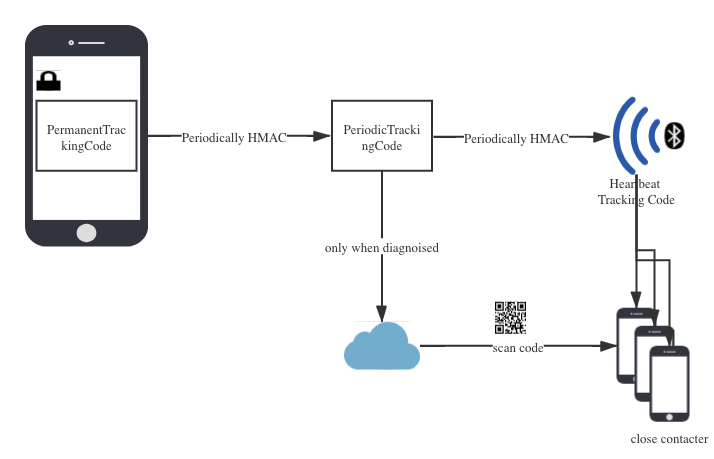
\includegraphics[width=0.7\linewidth]{figure/3phasecode}
	\caption{The 3 Code Interaction}
	\label{fig:fig1}
\end{figure}


\subsubsection{Inter-Device Communication}
In our protocol, the client use bluetooth low energy beacon \cite{liao2020correction, panther2017adaptive}to transmit Heartbeat Tracking Code to other closed receivers' clients. Bluethooth LE has a theoretical maximum distance/range of 100m, however the effective range is far less than that.

Similar to WiFi device discovery, the Contact Tracing is based on advertising, a.k.a. Bluetooth payloads that our device sends out to anyone within reach, and scanning, which is receiving and reading other devices advertisements.

No connection between devices is ever made: all devices will literally throw messages out in the air and read whatever comes in.

\subsubsection{Working Principle}
Let's assume that A is diagnosed. For example, the retrospective period is 14 days, and the Periodic Tracking Code of A's mobile phone in the past 14 days is used as a "diagnosis code" and uploaded to the cloud.

All users' mobile phones will download all the diagnosis codes of the diagnosed patients from the server when scanning or acquiring the health code, and then use the same encryption algorithm to calculate the Heartbeat Tracking Code locally.

Let's assume that in the past 14 days, A and B have been in the same room for a period of time, then the Heartbeat Tracking Code from A must be stored on B's mobile phone. If B's mobile phone is calculated, the obtained Periodic Tracking Code appears in the records kept by him for the past 14 days, and the contact tracking and verification is completed.

\section{Discussion}
\subsection{Security}
As the cloud server can only get the Periodic Tracking Data, which can not infer the metadata, so the cloud server can not read person's information. The Metadata Tracking Code or Temporary Exposure Key $tek$ are stored in the users' devices, which may contain some privacy information, It can not be acquired from the $aemk$ as we use $tek$ generate $aemk$ with $HKDF$. A government of this country has developed a tracking tool using this set of APIs. On the server side, administrators cannot know which other users a healthy user has contacted with—the administrator can only do so for diagnosed patients.

Also, the uploaded information does not include geographic location information and is strictly limited to the use of Bluetooth low energy beacons. The Heartbeat Tracking Code is bound to the Periodic Tracking Code. Even if there is a confirmed patient, the calculation of the diagnostic Heartbeat Tracking Code uploaded by it is only performed on other users' mobile phones, not on the server side.



\subsection{Properties and functionalities}

When the health code is green, the Periodic Tracking Data(aemk) will not be uploaded to server, other user can only get his heartbeat tracking data generated from AES-128 with aemk. No useful information will be revealed regarding the person.

The government can pin the location of suspicious person as Their location information can be obtained from Wechat, When Periodic Tracking Code is uploaded, it means the relative peoples' location data can be obtained from Wechat server.

Statistical data can be obtained as the number of Periodic Tracking Code is easily accessible. 

Information transferred between different parties is performed through bluetooth, But the data is encrypted with $aemk$. Without the Periodic Tracking Code, it does not make sense to obtain the Heartbeat Tracking Code.

The app can store Periodic Tracking of positive infected people's data in blockchain to maintain the data integrity. So the contacts can download it from the server. 

Due to the setting of Bluetooth broadcast and scanning intervals, and the length of each Heartbeat Tracking Code is only 32 bytes, this set of technology implementation is also more power-saving and storage space-saving\cite{aiello2009bluetooth}. Overall, its power consumption should not be very impressive, at least it will not reach the exaggerated Chengdu. Of course, the specific broadcast and scan interval can be set by the operator of the tracking tool.

\section{Conclusion}
In this article, we propose a tracking code based health code exchange protocol, and verified its security and functionalities. The server only records the tracking code of the positive infected person, and does not get privacy information from the code itself. The tracking code exchange based on bluetooth low energy beacon is high-efficiency and low-power. To a certain extent, it can play the role of epidemiological traceback and infection risk alert.

\bibliography{wpref}

\end{document}
